% 12pt: grandezza carattere
% a4paper: formato a4
% openright: apre i capitoli a destra
% twoside: serve per fare un
% documento fronteretro
% report: stile tesi (oppure book)
\documentclass[12pt,a4paper,openright,twoside]{report}

%libreria per scrivere in italiano
\usepackage[italian]{babel}

% libreria per accettare i caratteri
% digitati da tastiera come ?
% si può usare anche
% \usepackage[T1]{fontenc}
% però con questa libreria
% il tempo di compilazione
% aumenta
\usepackage[latin1]{inputenc}

% libreria per impostare il documento
\usepackage{fancyhdr}

% libreria per avere l'indentazione all'inizio dei capitoli, ...
\usepackage{indentfirst}

%libreria per mostrare le etichette
%\usepackage{showkeys}

% libreria per inserire grafici
\usepackage{graphicx}

% libreria per utilizzare font particolari ad esempio \textsc{}
\usepackage{newlfont}

% librerie matematiche
\usepackage{amssymb}
\usepackage{amsmath}
\usepackage{latexsym}
\usepackage{amsthm}

% librerie per mostrare il codice sorgente
\usepackage{listings, xcolor}
\renewcommand{\lstlistingname}{Codice sorgente}
\renewcommand{\lstlistlistingname}{Codici sorgenti}
% impostano i margini
\oddsidemargin=30pt
\evensidemargin=20pt

% serve per la sillabazione: tra parentesi vanno inserite come nell'esempio le parole
% che latex non riesce a tagliare nel modo giusto andando a capo.
\hyphenation{sil-la-ba-zio-ne pa-ren-te-si}

% comandi per l'impostazione della pagina, vedi il manuale della libreria fancyhdr per ulteriori delucidazioni
\pagestyle{fancy}\addtolength{\headwidth}{20pt}
\renewcommand{\chaptermark}[1]{\markboth{\thechapter.\ #1}{}}
\renewcommand{\sectionmark}[1]{\markright{\thesection \ #1}{}}
\rhead[\fancyplain{}{\bfseries\leftmark}]{\fancyplain{}{\bfseries\thepage}}
\cfoot{}

%comando per impostare l'interlinea
\linespread{1.3}

\begin{document}

\begin{titlepage}
% crea un ambiente libero da vincoli di margini e grandezza caratteri: si pu\`o modificare
% quello che si vuole, tanto fuori da questo ambiente tutto viene ristabilito

% elimina il numero della pagina
\thispagestyle{empty}

% imposta il margina superiore a 6.5cm
\topmargin=6.5cm

% incolonna la scrittura a destra
\raggedleft

% aumenta la grandezza del carattere a 14pt
\large

% emfatizza (corsivo) il carattere
\em

%\ldots lascia tre puntini
%\ldots

% va in una pagina nuova
\newpage

% non numera l'ultima pagina sinistra
\clearpage{\pagestyle{empty}\cleardoublepage}
\end{titlepage}

\pagenumbering{roman} % serve per mettere i numeri romani
\chapter*{Introduzione} % crea l'introduzione (un capitolo non numerato)

% imposta l'intestazione di pagina
\rhead[\fancyplain{}{\bfseries INTRODUZIONE}]{\fancyplain{}{\bfseries\thepage}}
\lhead[\fancyplain{}{\bfseries\thepage}]{\fancyplain{}{\bfseries INTRODUZIONE}}

% aggiunge la voce Introduzione nell'indice
\addcontentsline{toc}{chapter}{Introduzione}
% \ldots
Questo lavoro ha l'obiettivo di implementare sul simulatore Alchemist il modello ad agenti.

Alchemist \`e un meta-simulatore estendibile, ispirato alla chimica stocastica e adatto al calcolo pervasivo e ai sistemi distribuiti. Fornisce un meta-modello flessibile, sul quale gli sviluppatori legano le proprie astrazioni, realizzando un'incarnazione.

Gli agenti sono definiti come entit\`a autonome distribuite nello spazio ed in grado di interagire tra pari e con l'ambiente in cui sono posti.

Per creare l'incarnazione sar\`a necessario definire gli agenti mappando il loro modello su quello fornito da Alchemist.


% non numera l'ultima pagina sinistra
\clearpage{\pagestyle{empty}\cleardoublepage}

%crea l'indice
\tableofcontents

% imposta l'intestazione di pagina
\rhead[\fancyplain{}{\bfseries\leftmark}]{\fancyplain{}{\bfseries\thepage}}
\lhead[\fancyplain{}{\bfseries\thepage}]{\fancyplain{}{\bfseries INDICE}}

% non numera l'ultima pagina sinistra
\clearpage{\pagestyle{empty}\cleardoublepage}

% crea l'elenco delle figure
\listoffigures

% non numera l'ultima pagina sinistra
\clearpage{\pagestyle{empty}\cleardoublepage}

% crea l'elenco delle tabelle
%\listoftables

% non numera l'ultima pagina sinistra
\clearpage{\pagestyle{empty}\cleardoublepage}

%% % crea l'elenco dei codici sorgenti
 \lstlistoflistings
%%
%% % non numera l'ultima pagina sinistra
%% \clearpage{\pagestyle{empty}\cleardoublepage}

%-%-%-%-%-%-%-%-%-%-%-%-%-%-%-%-%-%-%-%-%-%-%-%-%-%-%-%-%-%-%-%-%-%-%-%-%-%-%-%-
\chapter{Alchemist}
% imposta l'intestazione di pagina
\lhead[\fancyplain{}{\bfseries\thepage}]{\fancyplain{}{\bfseries\rightmark}}
% mette i numeri arabi
\pagenumbering{arabic}
Alchemist fornisce un ambiente di simulazione sul quale \`e possibile sviluppare nuove incarnazioni, ovvero nuove definizioni di modelli implementati su di esso.

%++-++-++-++-++-++-++-++-++-++-++-++-++-++-++-++-++-++-++-++-++-++-++-++-++-++-
\section{Il meta-modello}\label{MetaModelloAlchemist}
Il meta-modello di Alchemist pu\`o essere compreso osservando la figura \ref{fig:alchemistModel}.
%crea l'ambiente figura;
\begin{figure}[h] % [h] sta per here, cioè la figura va qui
\begin{center} % centra nel mezzo della pagina la figura
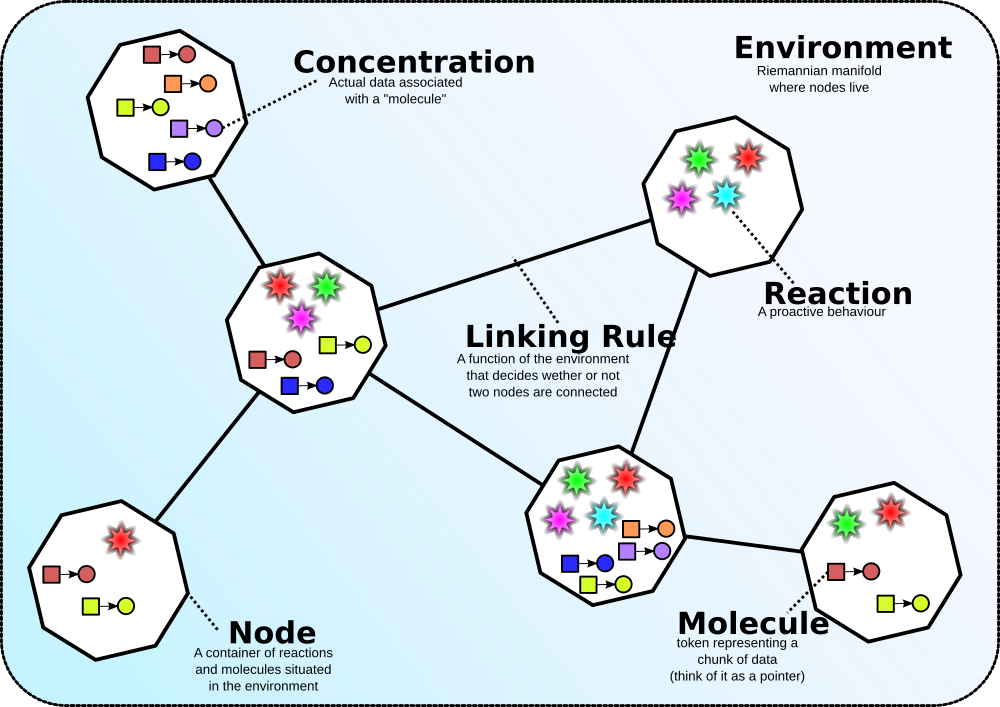
\includegraphics[width=12.5cm]{images/model.png} % inserisce una figura larga 12.5cm
% inserisce la legenda ed etichetta la figura con \label{fig:prima}
\caption[Illustrazione meta-modello di Alchemist]{Illustrazione meta-modello di Alchemist} \label{fig:alchemistModel}
\end{center}
\end{figure}

L'\textbf{\textit{Environment}} \`e l'astrazione dello spazio ed \`e anche l'entit\`a pi\`u esterna che funge da contenitore per i nodi. Conosce la posizione di ogni nodo nello spazio ed \`e quindi in grado di fornire la distanza tra due di essi e ne permette inoltre lo spostamento.

\`E detta \textbf{\textit{Linking rule}} una funzione dello stato corrente dell'environemnt che associa ad ogni nodo un \textbf{\textit{Vicinato}}, il quale \`e un entit\`a composta da un nodo centrale e da un set di nodi vicini.

Un \textbf{\textit{Nodo}} \`e un contenitore di molecole e reazioni che \`e posizionato all'interno di un environment.

La \textbf{\textit{Molecola}} \`e il nome di un dato, paragonabile a quello che rappresenta il nome di una variabile per i linguaggi imperativi.
Il valore da associare ad una molecola \`e detto \textbf{\textit{Concentrazione}}.

%crea l'ambiente figura;
\begin{figure}[h] % [h] sta per here, cioè la figura va qui
\begin{center} % centra nel mezzo della pagina la figura
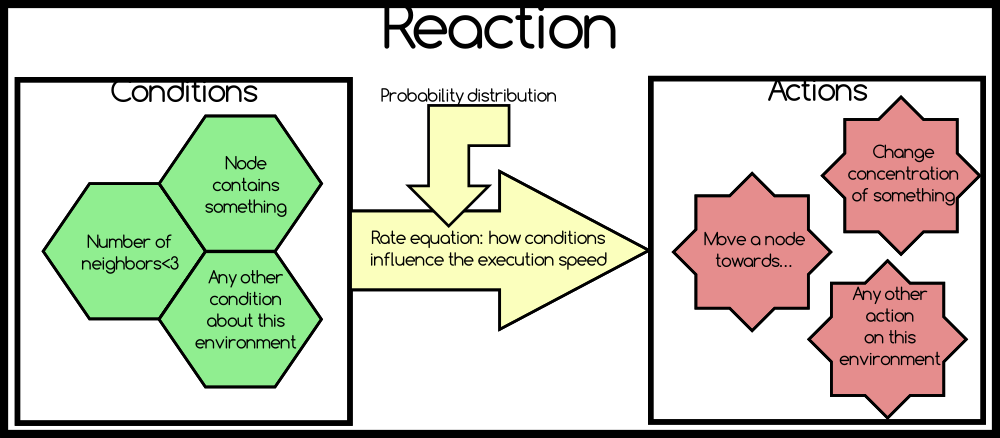
\includegraphics[width=14cm]{images/reaction.png} % inserisce una figura larga 12.5cm
% inserisce la legenda ed etichetta la figura con \label{fig:prima}
\caption[Illustrazione modello reazione di Alchemist]{Illustrazione modello reazione di Alchemist} \label{fig:alchemistReaction}
\end{center}
\end{figure}

Una \textbf{\textit{Reazione}} \`e un qualsiasi evento che pu\`o cambiare lo stato dell'environment ed \`e definita tramite una distribuzione temporale, una lista di condizioni e una o pi\`u azioni.
\\La frequenza con cui avvengono dipende da:
\begin{itemize}
\item un parametro statico di frequenza;
\item il valore di ogni condizione;
\item un'equazione di frequenza che combina il parametro statico e il valore delle condizioni restituendo la frequenza istantanea;
\item una distribuzione temporale.
\end{itemize}
Ogni nodo contiene un set di reazioni che pu\`o essere anche vuoto.

Per comprendere meglio il meccanismo di una reazione si pu\`o osservare la figura \ref{fig:alchemistReaction}.

Una \textbf{\textit{Condizione}} \`e una funzione che prende come input l'environment corrente e restituisce come output un booleano e un numero. Se la condizione non si verifica, le azioni associate a quella reazione non saranno eseguite. In relazione a parametri di configurazione e alla distribuzione temporale, una condizione potrebbe influire sulla velocit\`a della reazione.

La \textbf{\textit{Distribuzione temporale}} indica il numero di eventi, in un dato intervallo di tempo, generati da Alchemist e che innescano la verifica delle condizioni che possono portare alla potenziale esecuzione delle azioni.

Un'\textbf{\textit{Azione}} \`e la definizione di una serie di operazioni che modellano un cambiamento nel nodo o nell'environment.

In Alchemist un'incarnazione \`e un'istanza concreta del meta-modello appena descritta e che implementa una serie di componenti base come: la definizione di una molecola e del tipo di dati della concentrazione, un set di condizioni, le azioni e le reazioni. Incarnazioni diverse possono modellare universi completamente differenti.

%-%-%-%-%-%-%-%-%-%-%-%-%-%-%-%-%-%-%-%-%-%-%-%-%-%-%-%-%-%-%-%-%-%-%-%-%-%-%-%-
\chapter{Agenti}
% imposta l'intestazione di pagina
\lhead[\fancyplain{}{\bfseries\thepage}]{\fancyplain{}{\bfseries\rightmark}}

Un'agente \`e un entit\`a che agisce in modo autonomo e continuo in uno spazio condiviso con altri agenti e le sue caratteristiche principali sono: autonomia, proattivit\`a e reattivit\`a. Gli agenti sono formati da un nome, che \`e una caratteristica statica, e da componenti dinamici come lo stato.

%++-++-++-++-++-++-++-++-++-++-++-++-++-++-++-++-++-++-++-++-++-++-++-++-++-++-
\section{tuProlog}
tuProlog \`e un interprete Prolog per le applicazioni e le infrastrutture Internet basato su Java. \`E progettato per essere facilmente utilizzabile, leggero, configurabile dinamicamente, direttamente integrato in Java e facilmente interoperabile.

tuProlog \`e sviluppato e mantenuto da 'aliCE' un gruppo di ricerca dell'Alma Mater Studiorum - Universit\`a di Bologna, sede di Cesena. \`E un software Open Source e rilasciato sotto licenza LGPL.

Il motore tuProlog fornisce e riconosce i seguenti tipi di predicati:
\begin{itemize}
  \item predicati built-in: incapsulati nel motore tuProlog.
  \item predicati di libreria: inseriti in una libreria che viene caricata nel motore tuProlog. La libreria pu\`o essere liberamente aggiunta all'inizio o rimossa dinamicamente durante l'esecuzione. I predicati della libreria possono essere sovrascritti da quelli della teoria. Per rimuovere un singolo predicato dal motore \`e necesssario rimuovere tutta la libreria che contiene quel predicato.
  \item predicati della teoria: inseriti in una teoria che viene caricata nel motore tuProlog. Le teorie tuProlog sono semplicemente collezioni di clausole Prolog. Le teorie possono essere liberamente aggiunte all'inizio o rimosse dinamicamente durante l'esecuzione.
\end{itemize}

Librerie e teorie, pur essendo simili, sono gestite diversamente dal motore tuProlog.

\section{Agenti in tuProlog}
Gli agenti descritti in tuProlog sono entit\`a computazionali autonome che effettuano delle operazioni che impattano sul proprio stato e su quello dell'ambiente in cui sono immersi. La reattivit\`a \`e una caratteristica importante per quanto riguada gli agenti poich\`e fa si che siano pronti a reagire ad eventi o cambiamenti che avvengono nello spazio.
Un'agente \`e quindi definito attraverso una teoria, la quale \`e composta da regole che corrispondono ai piani dell'agente. I piani sono formati da una serie di operazioni volte a svolgere un'azione.

\section{Modello Jason}
Il modello di agenti a cui si fa riferimento in questo testo \`e quello utilizzato in Jason. Jason \`e un interprete, per la versione estesa di AgentSpeak, che implementa la semantica operazionale di tale linguaggio e fornisce una piattaforma per lo sviluppo di sistemi multi-agente. AgentSpeak, come appena accennato, \`e un linguaggio di programmazione orientato agli agenti basato sulla programmazione logica e l'architettura BDI.

Gli agenti BDI (Beliefs-Desires-Intentions) forniscono un meccanismo per separare le attivit\`a di selezione di un piano, fra quelli presenti nella sua teoria, dall'esecuzione del piano attivo, permettendo di bilanciare il tempo speso nella scelta del piano e quello per eseguirlo.

I \textbf{\textit{Beliefs}} sono informazioni dello stato dell'agente, ovvero ci\`o che l'agente sa del mondo (di se stesso e degli altri agenti), e possono comprendere regole di inferenza per permettere l'aggiunta di nuovi beliefs. L'insieme dei beliefs di un agente \`e detto 'belief base' o 'belief set' e si pu\`o modificare nel tempo.

I \textbf{\textit{Desires}} sono tutti i possibili piani che l'agente potrebbe eseguire. Rappresentano gli obiettivi o le situazioni che l'agente vorrebbe realizzare o portare a termine. I \textbf{goals} sono desires che l'agente persegue attivamente: per questo motivo, in generale, i piani desiderabili possono non essere coerenti tra loro mentre i goals \`e bene che lo siano.

Le \textbf{\textit{Intentions}} sono piani a cui l'agente ha deciso di lavorare o a cui sta gi\`a lavorando. I piani sono sequenze di azioni che un agente pu\`o eseguire per raggiungere una intention. I piani possono contenerne altri al loro interno.

Gli \textbf{\textit{Eventi}} innescano le attivit\`a reattive degli agenti il cui risultato pu\`o essere l'aggiornamento dei beliefs, la chiamata ad altri piani o la modifica di goals.


%-%-%-%-%-%-%-%-%-%-%-%-%-%-%-%-%-%-%-%-%-%-%-%-%-%-%-%-%-%-%-%-%-%-%-%-%-%-%-%-
\chapter{Progetto}
% imposta l'intestazione di pagina
\lhead[\fancyplain{}{\bfseries\thepage}]{\fancyplain{}{\bfseries\rightmark}}
Il progetto, come descritto nell'introduzione, ha come obiettivo l'approccio all'implementazione del meta-modello di Alchemist attraverso la definizione di un'incarnazione che modelli gli agenti all'interno del simulatore.

Per la realizzazione del ciclo di ragionamento dell'agente si \`e utilizzato il motore tuProlog importato e invocato all'interno del simulatore sfruttando la libreria 'aliCE'.


%++-++-++-++-++-++-++-++-++-++-++-++-++-++-++-++-++-++-++-++-++-++-++-++-++-++-
\section{Mapping dei modelli}
Il primo passo nell'evoluzione del progetto \`e stata l'analisi del mapping tra il meta-modello di Alchemist e il modello ad agenti, necessaria per individuare eventuali incongruenze o evidenziare opportunit\`a a livello applicativo e maggiore espressivit\`a.
Nei mapping effettuati si \`e cercato quindi di individuare l'entit\`a del meta-modello di Alchemist che offrisse maggiori opportunit\`a espressive per la definizione dell'agente.

Nella prima prova, l'agente \`e stato riferito ad un nodo, da cui ne deriva che l'environment sar\`a lo spazio che conterr\`a tutti gli agenti. Internamente al nodo, le molecole e le concentrazioni saranno utilizzate per gestire i beliefs dell'agente e le reazioni che saranno riferite ai piani utilizzando le condizioni come clausola per far scattare le azioni.
\\
Questo tipo di mapping consente di realizzare simulazioni di sistemi non complessi in cui vi \`e un solo 'livello' di agenti che interagiscono tra loro. Questa affermazione pu\`o essere compresa meglio analizzando il secondo tentativo che \`e stato effettuato.

Nel secondo mapping, l'agente \`e stato spostato pi\`u internamente al nodo riferendolo ad una reazione facendo diventare il nodo stesso uno spazio per gli agenti. In questo modo l'environment sar\`a uno spazio in cui possono essere presenti pi\`u nodi, i quali a loro volta potranno contenere un set di agenti.
\\
Utilizzando questo secondo caso si riuscir\`a a creare un sistema con pi\`u agenti all'interno di un singolo nodo, che in ambito applicativo pu\`o essere riferito ad un device, il quale si muover\`a nello spazio insieme ad altri nodi, contenitori di altri agenti.

La frequenza con cui gli eventi di Alchemist sono innescati dipende, oltre che dai parametri passati nella configurazione della simulazione, anche dalle condizioni definite per quello specifico agente: questo influisce sul numero di volte in cui viene eseguita un'azione, ovvero il ciclo di ragionamento dell'agente.

\section{Incarnazione}
L'incarnazione in Alchemist corrisponde all'implementazione del modello che si vuole realizzare espresso nella forma del meta-modello che \`e stato descritto nella sezione \ref{MetaModelloAlchemist}.
Dopo aver analizzato i due diversi mapping e le relative opportunit\`a implementative \`e stato scelto per implementare il modello ad agenti quello realizzato nella seconda analisi che riferisce l'agente ad una reazione.

Lo sviluppo \`e quindi partito dalla definizione della classe \textbf{AgentIncarnation} che implementa l'interfaccia \textit{Incarnation} nella quale sono definiti i metodi per la creazione delle entit\`a del meta modello (Molecola, Concentrazione, Nodo, Distribuzione temporale, Reazione, Condizione, Azione). Per oguna di quest'ultime verr\`a presentata qui di seguito la logica implementativa.

Per la realizzazione del \textbf{nodo}, che \`e l'entit\`a centrale del modello di Alchemist, \`e stata creata la classe \textbf{AgentsContainerNode} che estende la classe astratta \textit{AbstractNode}. All'interno del nodo, sono definite le propriet\`a per la memorizzazione del riferimento all'ambiente a cui appartiene e una mappa che memorizza gli agenti presenti al suo interno in coppie (\textit{nome\_agente}, \textit{oggetto\_agente}). Per quanto riguarda i metodi sono stati imlementati quelli dell'interfaccia e aggiunti altri per la gestione della mappa (inserimento agente e recupero dello stesso dalla mappa).

Per la \textbf{distribuzione temporale} \`e stata utilizzata la classe \textit{DiracComb}, gi\`a presente all'interno delle implementazioni di Alchemist, che permette la realizzazione di un pettine di Diract il cui spazio tra gli intervalli \`e definito dal parametro passato al costruttore. In questo caso il parametro \`e quello recuperato dalla configurazione della simulaizone poich\`e pu\`o variare per ogni specifica reazione.

Il metodo per la creazione delle \textbf{reazioni} viene invocato da Alchemist in base alla struttura del file di configurazione che specifica quali reazioni creare e in che nodo inserirle. Come visto precedentemente nella sezione \ref{MetaModelloAlchemist} le reazioni sono formate da condizioni e azioni, quest'ultime scatenate se si verificano le condizioni associate. La classe che definisce questa entit\`a \`e \textbf{AgentReaction} che estende la classe astratta \textit{AbstractReaction}. All'interno della classe \`e definita la propriet\`a per memorizzare il nome dell'agente e i metodi definiti nell'interfaccia.
Nel mapping realizzato la reazione si riferisce all'agente poich\`e ci\`o che la compone sono l'azione da scatenare e la clausola per innescarla ma l'agente vero e proprio, come vedremo successivamente, sar\`a implementato nelle azioni.

La \textbf{condizione} \`e creata utilizzando la classe \textit{AbstractCondition}, gi\`a definita nelle implementazioni di Alchemist, e che permette, attraverso i metodi rimasti da implementare, di definire la clausola che si deve verificare per scatenare le azioni di quella reazione.

Per la realizzazione delle \textbf{azioni} si \`e deciso di definire una classe astratta che racchiuda al suo interno le funzionalit\`a dell'agente cos\`i che le classi specifiche possano far eseguire all'agente solo le operazioni desiderate. Per fare ci\`o \`e stata creata la classe \textbf{AbstractAgent} che estende la classe astratta \textit{AbstractAction} non implementando i metodi \textit{cloneAction} e \textit{execute} in modo tale da lasciare la loro definizione alle classi specifiche. Le propriet\`a della classe creata sono relative al nome dell'agente e al motore tuProlog, all'interno del quale \`e caricata la libreria che definisce le regole da poter utilizzare.

Le entit\`a \textbf{molecola} e \textbf{concentrazione} sono state utilizzate solo per la tematizzazione delle simulazioni utilizzando come molecola il nome dell'agente e come valore 0. Associando, nel pannello della simulazione, colori diversi ad ogni nome la visione della simulaizone viene agevolata.

\medskip

Questa implementazione delle classi utilizzate all'interno dell'incarnazione \`e quella base; altri metodi e altre propriet\`a verranno aggiunte con la realizzazione delle funzionalit\`a specifiche, come vedremo successivamente.


\subsubsection{Referenziazione oggetti Java-tuProlog}
All'interno della classe \textbf{AbstractAgent}, come accennato precedentemente, sono implementate le funzionalit\`a da utilizzare nella definizione del ciclo di ragionamento che verr\`a descritto nella sezione \ref{CicloDiRagionamento}. Al suo interno sono stati utilizzati inoltre meccanismi per la referenziazione di oggetti Java all'interno di tuProlog, i quali consentono di effettuare invocazioni, dalla teoria dell'agente, di metodi definiti nelle classi Java. Per fare ci\`o sono stati registrati all'interno della teoria due variabili identificate con delle stringhe e riferite ad oggetti Java, una per il nodo (all'interno del quale \`e posizionato l'agente) e una per l'agente stesso.
\lstset{
  numberstyle=\footnotesize\color{black},
  basicstyle=\ttfamily,
  breakatwhitespace=true,
  breaklines=true,
  captionpos=b,
  keepspaces=true,
  numbers=left,
  numbersep=3pt,
  showspaces=false,
  showstringspaces=false,
  showtabs=false,
  tabsize=2,
  frame=tb,
  language=Java,
  commentstyle=\color{gray},
  keywordstyle=\color{blue},
  stringstyle=\color{red}
}
\medskip
\begin{lstlisting}[label={lst:ObjectReferenceJava},caption={Associazione riferimento oggetti Java per tuProlog}]
private final Library lib = this.engine.getLibrary("alice.tuprolog.lib.OOLibrary");
...
// Object reference for internal actions
((OOLibrary) this.lib).register(new Struct("agent"), this);
// Object reference for external actions
((OOLibrary) this.lib).register(new Struct("node"), this.getNode());
\end{lstlisting}

\section{Ciclo di ragionamento}\label{CicloDiRagionamento}
Il ciclo di ragionamento \`e il modo in cui l'agente prende le sue decisioni e mette in pratica le azioni.

%crea l'ambiente figura;
\begin{figure}[h] % [h] sta per here, cioè la figura va qui
\begin{center} % centra nel mezzo della pagina la figura
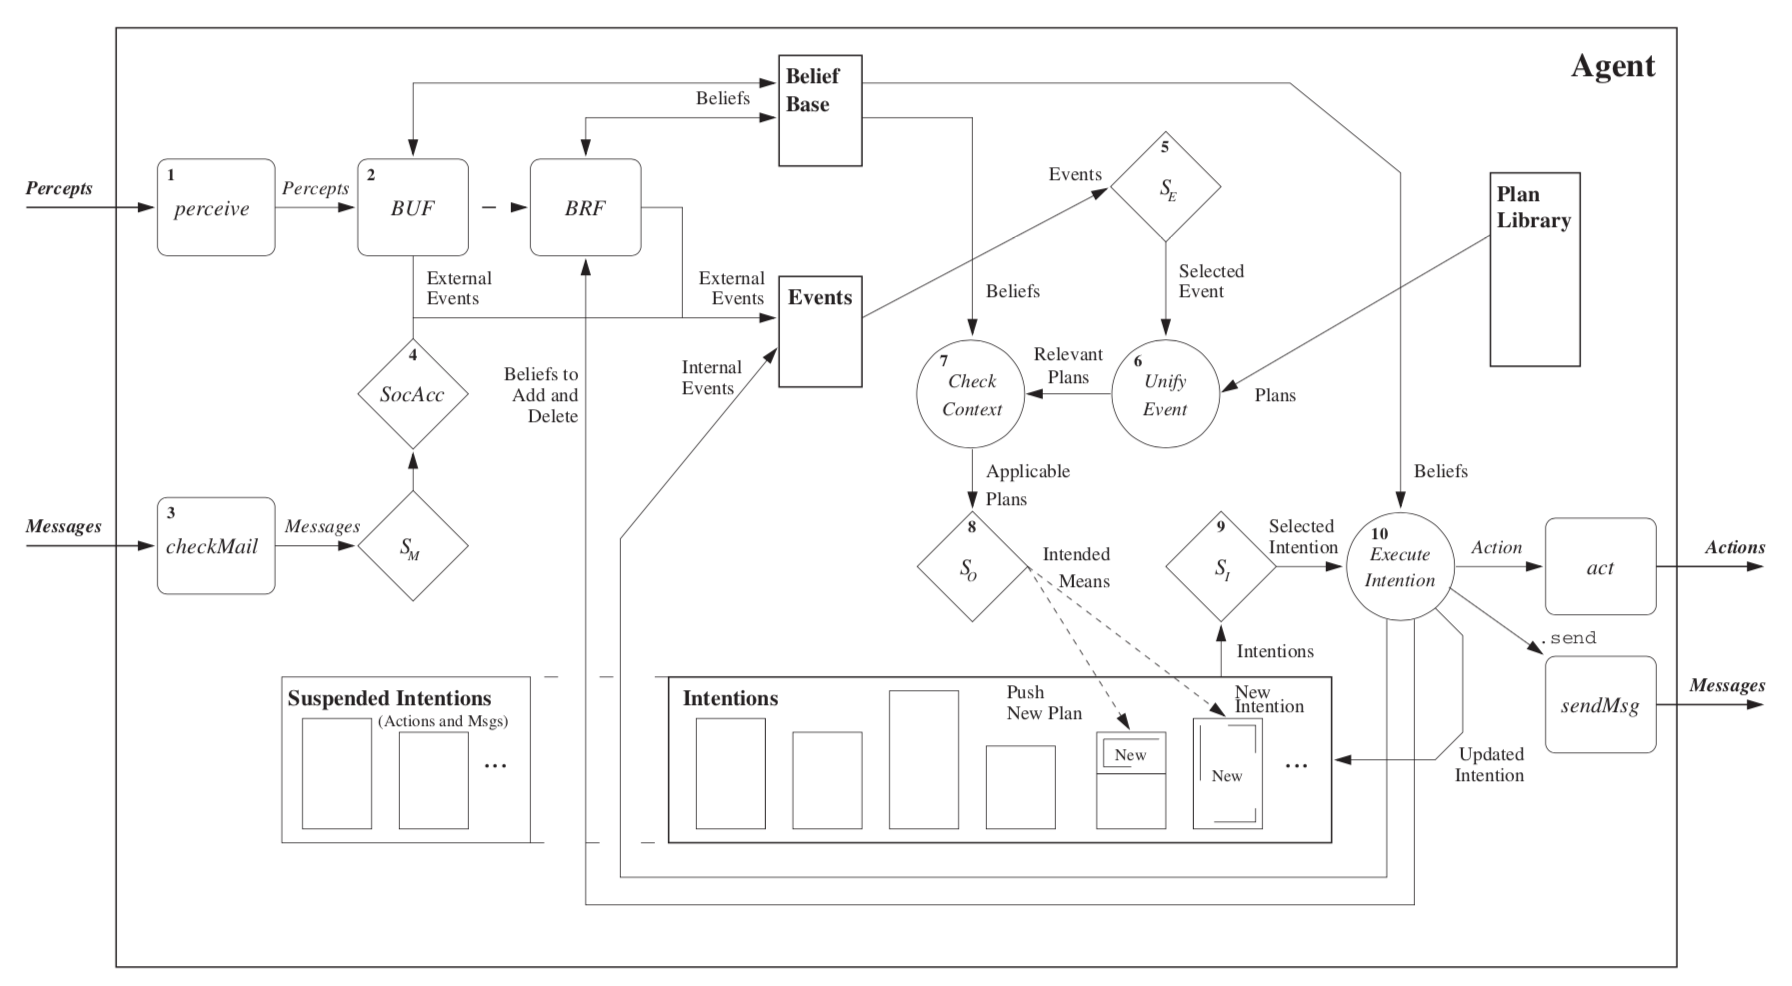
\includegraphics[width=16cm]{images/reasoningCicle.png} % inserisce una figura larga 12.5cm
% inserisce la legenda ed etichetta la figura con \label{fig:prima}
\caption[Ciclo di ragionamento di un agente]{Ciclo di ragionamento di un agente Jason} \label{fig:reasoningCicle}
\end{center}
\end{figure}

Per costruire il ciclo di ragionamento per gli agenti, da implementare all'interno di Alchemist, ci si \`e ispirati a quello proposto da Jason che \`e rappresentato in figura \ref{fig:reasoningCicle}.

\subsection{Ciclo di ragionamento in Jason}
Per comprendere meglio la rappresentazione del ciclo di ragionamento implementato in Jason (rappresentato in Figura \ref{fig:reasoningCicle}) qui di seguito sono spiegati i 10 step da cui \`e composto.
I rettangoli rappresentano lo stato dell'agente. I box arrotondati, i rombi e i cerchi rappresentano le funzioni usate nel ciclo di ragionamento: i primi due identificano funzioni che possono essere personalizzate dal programmatore, mentre i cerchi sono le parti fondamentali dell'interprete che non possono essre modificate. La differenza tra box arrotondati e rombi \`e che la funzione di quest'ultimi \`e di selezione: prendono in input una lista di elementi e la funzione ne sceglie uno.

Il ciclo di ragionamento sar\`a analizzato nei prossimi paragrafi suddividendolo in dieci step. Gli step 1-4 sono quelli che riguardano l'agente per l'aggiornamento dei suoi beliefs relaviti al mondo e agli altri agenti. Gli step 5-10 descrivono la parte principale: uno degli eventi viene selezionato per essere gestito e permettere l'esecuzione di un'intenzione dell'agente.


\subsubsection{(1) Percezione dell'ambiente}
La prima azione effettuata dall'agente all'interno del ciclo di ragionamento \`e la precezione di ci\`o che lo circonda, in modo da poter aggiornare i propri beliefs sullo stato dell'ambiente. L'agente deve utilizzare quindi dei componenti capaci di percepire l'ambiente ed essere interrogati dall'agente.
\\
In ambito applicativo l'agente acceder\`a ai dati dei sensori, prodotti da dispositivi del mondo reale, utilizzando le opportune interfacce.


\subsubsection{(2) Aggiornamento dei beliefs}
Ottenuta la lista delle percezioni \`e necessario aggiornare la 'belief base', ovvero l'insieme dei beliefs dell'agente. L'aggiornamento, descritto in figura \ref{fig:reasoningCicle} dall'acronimo 'BUF' (Belief Update Function), avviene nella seguente maniera: ogni percezione che non \`e gi\`a presente nella 'belief base' viene aggiunta e viceversa i beliefs che non sono nell'elenco delle percezioni vengono rimossi.
\\
Ognuno dei cambiamenti effettuati nell'aggiunta o rimozione di beliefs produce un evento: quelli generati da percezioni dell'ambiente sono chiaamti \textit{eventi esterni}. Gli \textit{eventi interni} hanno, in pi\`u rispetto agli altri eventi, associata un'intenzione.


\subsubsection{(3) Ricezione di comunicazioni da altri agenti}
Un'altra importante sorgente di informazioni per un agente in un sistema multi-agente sono gli altri agenti. L'interprete controlla i messaggi che sono arrivati alla casella dell'agente e li rende a lui disponibili: in un ciclo di ragionamento solamente un messaggio pu\`o essere processato. Per dare rilevanza a certi messaggi \`e necessario utilizzare una funzione di selezione (indicata in figura \ref{fig:reasoningCicle} da S\textsubscript{M}) che permette di aumentarne la priorit\`a. Di default viene utilizzata la politica FIFO (First In First Out).


\subsubsection{(4) Selezione dei messaggi 'Socialmente accettabili'}
Prima che i messaggi siano processati, passano all'interno di una selezione che determina se possono essere accettatti o meno dall'agente. In figura \ref{fig:reasoningCicle} \`e rappresentata dalla sigla 'SoccAcc'. L'implementazione di default accetta tutti i messaggi da tutti gli agenti. Sovrascrivendo questa funzione \`e possibile utilizzarla per far ricevere ad un agente solo certi messaggi piuttosto che altri.


\subsubsection{(5) Selezione di un evento}
Gli agenti BDI operano gestendo continuamente eventi, i quali rappresentano sia la precezione di cambiamenti nell'ambiente sia il cambiamento dei goal dello stesso agente.
\\
In ogni ciclo di ragionamento solo un evento pu\`o essere gestito. Ci possono essere vari eventi in attesa ma ne verr\`a selezionato solamente uno, il quale \`e scelto dalla funzione di selezione (indicata in figura \ref{fig:reasoningCicle} da S\textsubscript{E}). Il set di eventi \`e rappresentato da una lista e i nuovi eventi sono aggiunti in fondo: l'implementazione di base della funzione seleziona il primo elemento della lista, adottando quindi una politica FIFO.

I prossimi step considerano che un evento \`e stato selezionato e rimosso dalla lista di eventi in attesa. Se la lista di eventi fosse vuota, la selezione dell'evento non avverrebbe e il ciclo di ragionamento salterebbe allo step 9.

\subsubsection{(6) Recupero di tutti i paini rilevanti}
Selezionato l'evento, \`e necessario trovare un piano che permetta all'agente di agire in modo tale da gestire quell'evento. La prima cosa da fare \`e recuperare dalla 'Plan Library' i piani rilevanti, verificando quali tra questi abbia un evento di attivazione che pu\`o essere unificato con l'evento selezionato. L'unificazione \`e il confronto che viene fatto relativo a predicato e termini.
\\
Al fine di questo step si otterr\`a un set di piani rilevanti per l'evento selezionato e che nello step successivo verr\`a raffinato per ottenere il set di piani applicabili.


\subsubsection{(7) Determinazione dei piani applicabili}
Ogni piano ha un contesto che definisce se pu\`o essere usato in un certo momento in base alle informazioni che ha l'agente. In questo step si selezionano, tra i piani rilevanti, quelli che, in relazione alla situazione dell'agente, possono avere una possibilit\`a di successo. Per fare questo si controlla se il contesto \`e una coseguenza logica della 'belief base' dell'agente. Avere pi\`u di un piano nel set di quelli applicabili significa che in base alle conoscenza dell'agente e i suoi attuali beliefs qualsiasi di questi piani sarebbe appropriato per gestire l'evento.


\subsubsection{(8) Selezione di un piano applicabile}
Sebbene qualsiasi dei piani selezionati \`e adeguato, cio\`e l'esecuzione di uno di essi sar\`a sufficiente per gestire l'evento selezionato in questo ciclo di ragionamento, l'agente ne deve selezionarne solamente uno e impegnarsi ad eseguirlo. Vale a dire che l'agente avr\`a l'intenzione di perseguire l'azione determinata da quel piano e che quindi quest'ultimo sar\`a presto inserito nel set di quelli da eseguire.
\\
La selezione del piano \`e fatta da una funzione di selezione (indicata in figura \ref{fig:reasoningCicle} da S\textsubscript{O}). Ogni piano applicabile \`e considerato come una valida alternativa che l'agente ha per la gestione dell'evento. Un'evento rappresenta un particolare goal o un particolare cambiamento percepito nell'ambiente. I goal attualmente nel set degli eventi rappresentano desideri diversi che l'agente pu\`o scegliere di perseguire, mentre i piani applicabili, per uno di questi goal, rappresentano le diverse azioni che l'agente pu\`o eseguire per raggiungere quello specifico goal.
L'ordine con cui il piano \`e selezionato dalla funzione di selezione \`e determinato dall'ordine con cui sono scritti nel codice sorgente dell'agente o dall'ordine con cui sono comunicati all'agente.
\\
Ci sono due modi diversi per aggiornare il set delle intenzioni che dipendono dal fatto che l'evento selezionato sia interno (cambiamento nei goals) o esterno (cambiamento percepito nell'ambiente).
Se l'agente acquisisce una nuova informazione notificata dall'ambiente viene creata una nuova intenzione per l'agente. Ogni singola intenzione nel set delle intenzioni rappresenta un diverso punto di attenzione per l'agente. Nel prossimo step verr\`a descritto come una particolare intenzione \`e scelta per essere eseguita nel ciclo di ragionamento.
Per quello che riguarda gli eventi interni, essi sono creati quando l'agente ottiene un nuovo goal da raggiungere. Ci\`o significa che, prima che venga ripreso il corso dell'azione che ha generato l'evento, \`e necessario trovare ed eseguire fino al completamento un piano per raggiungere tale goal. In questo caso, non sono create nuove intenzioni ma una di quelle esistenti viene spostata in alto, il che forma una pila di piani che facilita l'interprete poich\`e l'intenzione da eseguire \`e quella pi\`u in alto.
\\
Quando un piano \`e scelto dalla libreria, viene creata un'istanza di quel piano per essere inserita nel set delle intenzioni: la libreria dei piani non viene modificata ma \`e l'istanza che viene manipolata dall'interprete.


\subsubsection{(9) Selezione di un intenzione per l'esecuzione}
Assumendo di avere un evento da gestire, fino a questo momento nel ciclo di ragionamento abbiamo ottenuto una nuova intenzione. Tipicamente un agente ha pi\`u di un'intenzione nel set di intenzioni, ognuna delle quali rappresenta un diverso punto di attenzione e che potrebbe essere eseguita nel prossimo step del ciclo di ragionamento. Ad ogni ciclo avviene l'esecuzione di una sola intenzione, tra quelle che sono in attesa pronte per essere eseguite. Anche in questo caso \`e utilizzata una funzione di selezione (indicata in figura \ref{fig:reasoningCicle} da S\textsubscript{I}). Dato che il raggiungimento di certi obiettivi sar\`a pi\`u urgente di altri, la scelta della prossima intenzione \`e molto importante per come l'agente operer\`a nell'ambiente.
Il meccanismo \`e di tipo 'round-robin', cio\`e ogni intenzione \`e selezionata a turno e, quando viene scelta, viene eseguita solamente un'azione. Come per gli eventi, il set di intenzioni \`e gestito con politica FIFO: viene preso il primo elemento della lista e, una volta eseguito, viene aggiunto nuovamente alla fine. In questo modo viene garantita un'attenzione equa a tutte le intenzioni.


\subsubsection{(10) Esecuzione di uno step di un'intenzione}
Un agente ha varie intenzioni che competono tra loro per essere eseguite. Nello step precedente abbiamo scelto l'intenzione da eseguire che non \`e altro che il corpo di un piano formato da una sequenza di formule: ogni formula eseguita viene rimossa dal corpo dell'istanza del piano.
L'intenzione viene sospesa fino a quando l'azione non viene eseguita, in attesa che l'effettore esegua l'azione e confermi al ragionatore se \`e stata eseguita o meno. L'intenzione sospesa, invece di essere restituita all'insieme di intenzioni, passa a un'altra struttura che memorizza tutte le intenzioni sospese che sono in attesa di un feedback dell'azione o di un messaggio: certi tipi di comunicazione richiedono che l'agente attenda una risposta prima che tale intenzione possa essere ulteriormente eseguita. Dato che un agente ha varie intenzioni e nuovi eventi da gestire, anche se alcune delle intenzioni sono attualmente sospese, nel prossimo ciclo di ragionamento ci sar\`a sicuramente qualche altra intenzione da eseguire.

\subsection{Ciclo di ragionamento in Alchemist}
Il ciclo di ragionamento in Figura \ref{fig:reasoningCicle} \`e ci\`o che si \`e cercato di replicare per definire quello usato in questo progetto.
Ad ogni iterazione del ciclo l'agente deve essere in grado di:
\begin{itemize}
   \item percepire le modifiche dell'ambiente che lo circonda
   \item ricevere i messaggi e selezionarne uno da leggere (metodologia FIFO)
   \item aggiornare la 'belief base'
   \item selezionare un'intenzione da perseguire (metodologia Round-Robin)
   \item eseguire la prima operazione dello stack dell'intenzione selezionata e riaggiungere l'intenzione alla coda.
\end{itemize}

Per poter gestire le intenzioni sono stati previsti una serie di meccanismi sia lato Alchemist che lato tuProlog. All'interno della classe \textit{AbstracAgent} un'array contente gli identificativi delle intenzioni e le funzioni per crearle, rimuoverle e selezionarle per l'esecuzione mentre in tuProlog, attraverso apposite regole, viene gestita l'esecuzione delle operazioni che la compongono.

\subsubsection{Crezione intenzione}
Nel momento in cui Alchemist riceve un'evento da notificare all'agente, viene costruito un apposito fatto ed attraverso l'utilizzo del predicato \textit{clause(Head, Body)} che permette di recuperare il corpo di una regola conoscendo la sua testa. Se ci fossero pi\`u alternative disponibili, vengono tutte recuperate e da ognuna si ottiene la lista di operazioni che compongono il corpo da cui verr\`a generata l'intenzione.

\medskip

La creazione di un'intenzione segue questo processo:
\begin{itemize}
   \item recupero lista di operazioni per una certa intenzione
   \item generazione di un identificativo univoco
   \item creazione del fatto \textit{intention(Id,ListaOperazioni)}
   \item inserimento dell'id nello stack lato Java e del fatto all'interno della teoria tuProlog
\end{itemize}

Per ogni evento si avr\`a quindi una corrispondente intenzione che, come spiegato precedentemente, verr\`a eseguita periodicamente fino alla sua conclusione.

\subsubsection{Selezione e avvio esecuzione intenzione}
Ad ogni ciclo di ragionamento, dopo aver creato le intenzioni per gli eventi occorsi, si passa alla selezione dell'intenzione che deve essere eseguita. Per garantire ad ognuna equa possibilit\`a viene utilizzato il meotodo Round-Robin, che prevede l'utilizzo di un 'token' circolare che viene passato virtualmente tra gli elementi e chi ne \`e in possesso pu\`o compiere un'azione, in questo caso sarebbe l'esecuzione di un'operazione.
L'implementazione \`e effettuata tramite l'utilizzo di un array al quale viene prelevato l'elemento di testa e che poi una volta eseguito viene riaggiunto in coda.
Per avviare l'esecuzione e passare il controllo alla teoria viene risolto tramite il motore tuProlog \textit{execute(IntentionID)}.

\subsubsection{Gestione esecuzione intenzione}
Per la gestione dell'esecuzione delle intenzioni lato tuProlog sono state definite una serie di regole all'interno della libreria base dell'agente caricata nella classe \textit{AbstracAgent}.
Nella sezione precedente \`e stato selezionato l'identificativo dell'intenzione da eseguire, la quale poi viene scatenata. Nella libreria dell'agente sono presenti due regole che hanno come testa \textit{execute(IntentionID)} ma corpi differenti per due diverse risoluzioni: la definizione \`e mostrata nel Codice sorgente \ref{lst:EsecuzioneIntenzione}.
\lstset{
  numberstyle=\footnotesize\color{black},
  basicstyle=\ttfamily,
  breakatwhitespace=false,
  breaklines=true,
  captionpos=b,
  keepspaces=true,
  numbers=left,
  numbersep=0pt,
  showspaces=false,
  showstringspaces=false,
  showtabs=false,
  tabsize=2,
  frame=tb,
  commentstyle=\color{black},
  keywordstyle=\color{black},
  stringstyle=\color{black}
  %label=incarnationYAML,
  %caption={First verbatim}
  %language=Java
  %escapeinside={(*@}{@*)}
}
\medskip
\begin{lstlisting}[firstnumber=1,label={lst:EsecuzioneIntenzione},caption={Regole per l'esecuzione dell'intenzione}]
   execute(I) :-
      intention(I, []),
      !,
      agent <- removeCompletedIntention(I).

   execute(I) :-
      retract(intention(I, [ACTION | STACK])),
      execute(I, ACTION, TOP),
      !,
      append(TOP, STACK, NEWSTACK),
      assertz(intention(I, NEWSTACK)).
\end{lstlisting}
Le due regole mostrate operano, come appena detto, due azioni diverse. La prima recupera il fatto dell'intenzione utilizzando l'identificativo e una lista vuota: se va a successo vuol dire che l'intenzione selezionata non ha pi\`u operazioni nel suo stack e quindi pu\`o essere eliminata. Ed infatti, attraverso l'oggetto Java dell'agente, referenziato nella variabile \textit{agent} in tuProlog, viene invocato il metodo per cancellarla. Questo metodo elimina l'identificativo dallo stack lato Alchemist e poi rimuove il fatto dalla teoria.
Nella seconda regola, invece, viene rimosso il fatto relativo all'identificativo dell'intenzione e recuperato lo stack delle operazioni scomponendolo in testa e coda, rispettivamente 'ACTION' e 'STACK'. Successivamente viene richiamata l'esecuzione dell'azione in testa, la cui eventuale sequenza di operazioni innescata dalla sua esecuzione viene restituita nella variabile 'TOP'. Quest'ultima viene quindi concatenata alla coda ('STACK') in modo tale che le prossime volte che l'intenzione viene selezionata le operazioni vengano eseguite.

Essendo l'ordine importante, come si pu\`o vedere dal codice mostrato, viene prima inserita la regola per la rimozione e successivamente quella per effettuare l'esecuzione delle azioni.

\subsubsection{Gestione esecuzione azioni}
Fino ad ora \`e stato mostrato come \`e stata implementata la gestione delle intenzioni, sia lato Alchemist (Java) che lato tuProlog, e la loro esecuzione ma non sono state descritte le azioni che le compongono.
Le tipologie di azioni che sono state implementate sono interne ed esterne. Quelle interne sono azioni che hanno impatto internamente all'agente e sono definite nell'implementazione della sua classe. Invece, quelle esterne, hanno impatto sull'ambiente e vengono gestite dal nodo che, per l'implementazione creata, \`e sia l'elemento inserito nell'ambiente sia esso stesso uno spazio per gli agenti posizionati al suo interno.

Un'altra differenziazione che si pu\`o fare \`e quella tra le varie tipologie di goal definite: achievement, test, concurrent. Relativamente al mondo Jason sono riferiti rispettivamente ai simboli '!', '?' e '!!' o '!?' e stanno ad indicare i goal, ovvero operazioni 'prioritarie' rispetto ad altre.

\section{Funzionalit\`a agente}
All'interno del ciclo di ragionamento implementato nella classe specifica dell'agente possono essere richiamate le funzionalit\`a definite nella classe astratta oppure altre definite localmente.
Nell'attuale implementazione dell'incarnazione, nella classe \textit{AbstracAgent} sono state definite funzioni per lo scambio di messaggi tra agenti, lo spostamento del nodo in cui sono posizionati gli agenti, la notifica dell'aggiornamento (inserimento o rimozione) della 'belief base'.

Nelle prossime sezioni sono mostrate le implementazioni delle funzionalit\`a appena descritte.

\subsection{Scambio di messaggi}
Per la realizzazione dello scambio di messaggi tra agenti si \`e modificata la classe \textbf{AbstractAgent} inserendo due code per i messaggi, una per quelli in entrata e una per quelli in uscita, e i relativi metodi per la loro gestione (lettura e inserimento in entrambe le code).

Le due code sono state realizzate utilizzando oggetti di tipo \textit{Queue} e istanziati come \textit{LinkedList}: una lista conterr\`a i messaggi in entrata mentre l'altra quelli in uscita. Per gestire meglio i messaggi sono state create due classi InMessage e OutMessage, dove la prima si riferisce a quelli ricevuti mentre la seconda a quelli inviati. Entrambe sono state definite all'interno della classe \textbf{AbstractAgent}.
La classe InMessage ha al suo interno le propriet\`a sender e payload usate per descrivere rispettivamente il mittente e il contenuto del messaggio.
La classe OutMessage contiene le propriet\`a sender, receiver e payload per descrivere il mittente, il destinatario e il contenuto del messaggio.
In entrambe le classi sono definiti solo i metodi getter poich\`e le propriet\`a sono assegnate solo nel costruttore della classe.

La gestione delle code tramite i metodi avviene secondo la politica FIFO, quindi l'inserimento \`e fatto in coda e la rimozione dalla testa. Come avviene la consegna dei messaggi vera e propria verr\`a spiegato successivamente nella sezione \ref{ConsegnaMessaggi}.

Inizialmente sia la lettura che la scrittura erano gestite effettuando chiamate tramite il motore tuProlog per inserire o recuperare i messaggi nelle code ed anche per la loro lettura. Dopo la rifattorizzazione e l'inserimento degli oggetti Java all'interno della teoria l'implementazione \`e stata semplificata permettendo una gestione pi\`u snella.

Per la \textbf{lettura dei messaggi} \`e stato definito il metodo \textit{readMessage}, il quale pu\`o essere inserito nel ciclo di ragionamento per permetter all'agente di gestire i messaggi ricevuti.
All'interno del metodo viene recuperato, se presente, il primo messaggio della coda e successivamente viene composto il predicato 'onReceiveMessage(S,M)' dove S \`e il mittente e M \`e il contenuto del messaggio.
Attraverso l'utilizzo del motore tuProlog, il predicato appena descritto viene eseguito nella teoria dell'agente che se opportunamente programmata pu\`o essere in grado di ricevere il messaggio ed operare di conseguenza.

L'\textbf{invio di messaggi} viene scatenato dalla teoria tramite cosiddetta un'azione interna. Le azioni interne sono azioni che hanno luogo internamente all'agente e, in questo caso, prevede l'inserimento di un messaggio nella coda di quelli in uscita.
L'azione interna prima di essere invocata passa per due controlli: il primo avviene nella teoria dell'agente e il secondo nel metodo di disambiguazione definito in Alchemist.
Nella teoria dell'agente il controllo avviene verificando la presenda di predicati del tipo 'is\_internal(ACTION)' dove 'ACTION' \`e l'azione da eseguire. Nel caso specifico controller\`a dell'esistenza del predicato 'is\_internal(iSend(S,M))': in caso positivo verr\`a eseguita l'operazione definita nel Codice sorgente \ref{lst:InvocazioneEsecuzioneAzioneInterna} per innescare l'azione lato Java.
\lstset{
  numberstyle=\footnotesize\color{black},
  basicstyle=\ttfamily,
  breakatwhitespace=false,
  breaklines=true,
  captionpos=b,
  keepspaces=true,
  numbers=left,
  numbersep=3pt,
  showspaces=false,
  showstringspaces=false,
  showtabs=false,
  tabsize=2,
  frame=tb,
  commentstyle=\color{black},
  keywordstyle=\color{black},
  stringstyle=\color{black}
  %label=incarnationYAML,
  %caption={First verbatim}
  %language=Java
  %escapeinside={(*@}{@*)}
}
\medskip
\begin{lstlisting}[label={lst:InvocazioneEsecuzioneAzioneInterna},caption={Invocazione esecuzione azione interna}]
agent <- executeInternalAction(ACTION)
\end{lstlisting}

\subsubsection{Consegna dei messaggi}\label{ConsegnaMessaggi}
Fino a questo momento gli agenti sono in grado di leggere messaggi presenti nella coda in entrata oppure inserirne di nuovi nella coda di quelli in uscita. La parte mancante \`e quella della consegna dei messaggi in uscita ai rispettivi destinatari. Per fare ci\`o si \`e pensato di creare un'apposito agente e definire una classe specifica, la classe \textbf{PostmanAgent}. L'agente Postman, che deve essere instanziato in configurazione, implementa la classe AbstracAgent come descritto nel Codice sorgente \ref{lst:PostmanAgent}. I metodi definiti al suo interno sono:
\begin{itemize}
   \item il costruttore, diversamente dagli altri agenti non viene passata la reazione
   \item cloneAction, definito nell'interfaccia Action, per clonare l'azione
   \item execute, definito nell'interfaccia Action, si riferisce al ciclo di ragionamento
\end{itemize}
\lstset{
  numberstyle=\footnotesize\color{black},
  basicstyle=\ttfamily,
  breakatwhitespace=true,
  breaklines=true,
  captionpos=b,
  keepspaces=true,
  numbers=left,
  numbersep=3pt,
  showspaces=false,
  showstringspaces=false,
  showtabs=false,
  tabsize=2,
  frame=tb,
  language=Java,
  commentstyle=\color{gray},
  keywordstyle=\color{blue},
  stringstyle=\color{red}
}
\medskip
\begin{lstlisting}[label={lst:PostmanAgent},caption={Agente Postman}]
public PostmanAgent(String name, Node node, RandomGenerator rand) {
   super(name, node, rand);
}

@Override
public Action cloneAction(Node node, Reaction reaction) {
   return new PostmanAgent("cloned_" + this.getAgentName(), node, this.getAgentRandomGenerator());
}

@Override
public void execute() {
   getNode().postman();
}
\end{lstlisting}
Come \`e possibile osservare, nel suo ciclo di ragionamento l'agente Postman non fa altro che eseguire l'azione postman definita nel nodo ed implementata come descritto nel Codice sorgente \ref{lst:PostmanMethod}.
Inizialmente vengono create una mappa di appoggio per gli agenti e una lista dei messaggi in uscita.
Per ogni nodo viene recuperata la sua mappa di agenti, quelli contenuti al suo interno, e viene aggiunta a quella temporanea, la quale viene poi iterata per recuperare tutti i messaggi in uscita da ogni agente aggiunti alla lista creata in precedenza.
Una volta ottenuti i messaggi viene iterata la lista e, utilizzando la mappa degli agenti creata in precedenza per recuperare l'istanza del destinatario di ogni messaggio, viene inserito invocato il metodo \textit{addIncomingMessage} che aggiunge un messaggio alla coda di quelli in entrata per quell'agente.
\medskip
\begin{lstlisting}[label={lst:PostmanMethod},caption={Metodo dell'agente Postman}]
Map<String, AbstractAgent> tmpAgentMap = new LinkedHashMap<>();
List<AbstractAgent.OutMessage> outMessages = new ArrayList<>();

// For each node in the environment get all its agents
this.environment.getNodes().forEach(node -> {
   tmpAgentMap.putAll(((AgentsContainerNode) node).getAgentsMap());
});

// For each agent takes outgoing messages
tmpAgentMap.forEach((agentName, agent) -> {
   outMessages.addAll(agent.consumeOutgoingMessages());
});

// Send each message to the receiver
outMessages.forEach(message -> {
   tmpAgentMap.get(message.getReceiver().toString())
   .addIncomingMessage(message);
});
\end{lstlisting}

\subsection{Spostamento del nodo}
Per lo spostamento del nodo all'interno dello spazio si \`e deciso di modificare la classe \textbf{AgentsContainerNode} aggiungendo tre propriet\`a per memorizzare direzione, velocit\`a e il tau (tempo della simulazione) dell'ultimo aggiornamento. Inoltre sono stati definiti i metodi per recuperare e impostare i valori della velocit\`a e della direzione.
Per quanto riguarda l'aggiornamento della posizione \`e stato definito il metodo \textit{changeNodePosition(Time updateTau)} che prende in input il tau dell'aggiornamento.
questo metodo \`e implementato come mostrato dal Codice sorgente \ref{lst:AggiornamentoPosizioneNodo}.
Questo metodo \`e quindi responsabile di calcolare la nuova posizone del nodo utilizzando le propriet\`a descritte in precedenza. Per prima cosa viene recuperata la posizione corrente del nodo che viene utilizzata come centro per la costruzione di una circonferenza, la quale avr\`a come raggio la distanza calcolata moltiplicando la velocit\`a per il tempo trascorso dall'ultimo aggiornamento. La nuova posizione del nodo si trover\`a dunque sulla circonferenza e per selezionare il punto viene utilizzata la direzione, espressa in radianti.
\medskip
\begin{lstlisting}[label={lst:AggiornamentoPosizioneNodo},caption={Metodo per l'aggiornamento della posizione del nodo}]
Position currentPosition = this.getNodePosition();
double radAngle = this.nodeDirectionAngle;
// radius = space covered = time spent * speed
double radius = (updateTau.toDouble() - this.lastUpdateTau.toDouble()) * this.nodeSpeed;
double x = currentPosition.getCoordinate(0) + radius * Math.cos(radAngle);
double y = currentPosition.getCoordinate(1) + radius * Math.sin(radAngle);

this.environment.moveNodeToPosition(this, this.environment.makePosition(x, y));
this.lastUpdateTau = updateTau;
\end{lstlisting}

Inizialmente l'aggiornamento era stato inserito erroneamente nel ciclo di ragionamento dell'agente. \`E stato rimosso quando ci si \`e resi conto che cos\`i facendo, in caso di pi\`u agenti all'interno dello stesso nodo, la posizione veniva aggiornata molteplici volte ed ognuna con parametri diversi poich\`e direzione e velocit\`a possono essere modificate costantemente.
A seguito di un'analisi, \`e stato deciso di creare un agente specifico per l'aggiornamento della posizione inserito direttamente nel codice, diversamente dall'agente Postman che deve essere aggiunto nella configurazione della simulazione.
L'agente appena descritto \`e definito dalla classe \textbf{MovementAgent}, la cui implementazione \`e praticamente identica a quella dell'agente Postman se non per il comportamento nel ciclo di ragionamento.
Nel metodo \textit{execute}, come si pu\`o osservare dal Codice sorgente \ref{lst:MovementAgent}, effettua due invocazioni di metodi definiti nella classe del nodo: la prima per l'aggiornamento della posizione al metodo descritto nel Codice sorgente \ref{lst:AggiornamentoPosizioneNodo} e la seconda per aggiornare i belief della distanza dagli altri agenti presenti nelle teorie.
L'aggiornamento della posizione avviene utilizzando i valori di velocit\`a e direzione presenti in quel momento. \`E quindi chiaro che se vi fossero pi\`u agenti che modifichino quelle propriet\`a solo le ultime impostate saranno quelle effettivamente utilizzate.
\medskip
\begin{lstlisting}[label={lst:MovementAgent},caption={Agente per lo spostamento del nodo}]
public MovementAgent(String name, Node node, RandomGenerator rand, Reaction reaction) {
   super(name, node, rand, reaction);
}

@Override
public Action cloneAction(Node node, Reaction reaction) {
   return new MovementAgent("cloned_" + this.getAgentName(), node, this.getAgentRandomGenerator(), reaction);
}

@Override
public void execute() {
   this.getNode().changeNodePosition(
      this.getAgentReaction().getTau());

   this.getNode().updateAgentsPosition();
}
\end{lstlisting}

Questo agente viene aggiunto alla creazione di ogni nodo: \`e quindi creata una reazione, chiamata 'movementReact', alla quale viene aggiunta la stessa condizione utilizzata per gli altri agenti e come azione l'agente appena definito. La reazione \`e definita con una distribuzione temporale di 1 tau, in modo tale che se si vuole simulare l'aggiornamento della posizione, come se arrivasse da un apparato GPS, sar\`a sufficiente impostare valori pi\`u altri per le distribuzioni temporali di altri agenti.
Terminata la creazione, la reazione viene aggiunta al nodo che verr\`a poi popolato con altri agenti. In questo modo la funzionalit\`a dello spostamento del nodo \`e implicita nell'incarnazione ed \`e il programmatore dell'agente che la pu\`o sfruttare implementando opportunamente gli agenti.

\subsection{Aggiornamento della 'belief base'}
Per quanto riguarda l'aggiornamento delle 'belief base' si \`e pensato di incapsulare i predicati 'asserta', 'assertz' e 'retract' utilizzando strutture dati e piani tuProlog per svolgere lo stesso comportamento: modifica della 'belief base', notifica del cambiamento tramite evento. In questo modo si \`e in grado di spezzare l'inserimento o la rimozione del belief dalla notifica del cambiamento, evitando che un agente operi un ciclo di ragionamento senza mai terminare, ovvero che l'agente continui a svolgere compiti lato tuProlog senza far tornare il controllo ad Alchemist.
\lstset{
  numberstyle=\footnotesize\color{black},
  basicstyle=\ttfamily,
  breakatwhitespace=false,
  breaklines=true,
  captionpos=b,
  keepspaces=true,
  numbers=left,
  numbersep=0pt,
  showspaces=false,
  showstringspaces=false,
  showtabs=false,
  tabsize=2,
  frame=tb,
  commentstyle=\color{black},
  keywordstyle=\color{black},
  stringstyle=\color{black}
  %label=incarnationYAML,
  %caption={First verbatim}
  %language=Java
  %escapeinside={(*@}{@*)}
}
\medskip
\begin{lstlisting}[firstnumber=1,label={lst:BeliefBaseUpdate},caption={Piani per l'aggiornamenot della 'belief base'}]
   addBelief(B) :-
     assertz(belief(B)),
     assertz(added_belief(B)).

   removeBelief(B) :-
     retract(belief(B)),
     assertz(removed_belief(B)).
\end{lstlisting}
I piani, definiti nella teoria, che permettono questo comportamento, sono mostrati nel Codice sorgente \ref{lst:BeliefBaseUpdate}.
L'aggiornamento della 'belief base' inizia con un'invocazione, da parte dell'agente, di uno di questi due piani che porta all'aggiunta del belief e di un secondo belief fittizio.
Lato Alchemist, durante il suo ciclo di ragionamento, l'agente invoca il metodo \textit{beliefBaseChanges()} implementato nella classe \textbf{AbstractAgent}.
All'interno del metodo vengono ritirati uno ad uno i belief fittizi inseriti in precedenza e poi per ognuno viene eseguito il piano 'onAddBelief(B)' o 'onRemoveBelief(B)', dove B \`e il belief modificato, a seconda che il belief recuperato sia rispettivamente di aggiunta o di rimozione.

%-%-%-%-%-%-%-%-%-%-%-%-%-%-%-%-%-%-%-%-%-%-%-%-%-%-%-%-%-%-%-%-%-%-%-%-%-%-%-%-

\section{Simulazione}
Attraverso la configurazione e l'esecuzione delle simulazioni \`e possibile vedere il comportamento delle incarnazioni definite all'interno di Alchemist. Nelle prossime sezioni verr\`a mostrato quali sono le parti che compongono la configurazione di una simulazione e qual \`e la configurazione scelta.

%++-++-++-++-++-++-++-++-++-++-++-++-++-++-++-++-++-++-++-++-++-++-++-++-++-++-
\subsection{Scrivere una simulazione}
% style for general source code
\lstset{
  numberstyle=\footnotesize\color{black},
  basicstyle=\ttfamily,
  breakatwhitespace=false,
  breaklines=true,
  captionpos=b,
  keepspaces=true,
  numbers=left,
  numbersep=0pt,
  showspaces=false,
  showstringspaces=false,
  showtabs=false,
  tabsize=2,
  frame=tb
  %label=incarnationYAML,
  %caption={First verbatim}
  %language=Java
  %escapeinside={(*@}{@*)}
}
Il linguaggio da utilizzare per scrivere le simulazioni in Alchemist \`e YAML e quello che il parser del simulatore si aspetta in input \`e una mappa YAML.
\\
Nei prossimi paragrafi verr\`a mostrato quali sezioni si possono inserire e come utilizzarle per creare la simulazione che si vuole realizzare.

La sezione \textbf{incarnation} \`e obbligatoria. Il parser YAML si aspetta una stringa che rappresenta il nome dell'incarnazione da utilizzare per la simulazione.
\medskip
\begin{lstlisting}[firstnumber=last,caption={Incarnazione}]
  incarnation: agent
\end{lstlisting}

Nel resto della sezione, il valore associato alla chiave 'type' fa riferimento al nome di una classe. Se il nome passato non \`e completo, ovvero non \`e comprensivo del percorso fino alla classe, Alchemist provveder\`a a cercare la classe tra i packages.

Per dichiarare variabili che poi potranno essere richiamate all'interno del file di configurazione della simulazione si pu\`o procedere in questo modo.
\medskip
\begin{lstlisting}[firstnumber=last,caption={Variabili simulazione}]
  variables:
    myVar: &myVar
      par1: 0
      par2: "string"
    mySecondVar: &myVar2
      par: "value"
\end{lstlisting}

Utilizzando la keyword \textbf{environment} si pu\`o scegliere quale definizione di ambiente utilizzare per la simulazione.
\medskip
\begin{lstlisting}[firstnumber=last,caption={Environment}]
  environment:
    type: OSMEnvironment
    parameters: [/maps/foo.pbf]
\end{lstlisting}
Questo parametro \`e opzionale e di default \`e uno spazio continuo bidimensionale: ometterlo equivale a scrivere la seguente configurazione.
\medskip
\begin{lstlisting}[firstnumber=last,caption={Default environment}]
  environment:
    type: Continuous2DEnvironment
\end{lstlisting}

La keyword \textbf{positions} consente di specificare il tipo delle coordinate della simulazione. La psizione riflette lo spazio fisico: per esempio non si potr\`a utilizzare la distanza \textit{Continuous2DEuclidean} se si considera la mappa di una citt\`a visto che dati due punti A e B, nel mondo reale la distanza AB \`e diversa da quella BA.
\medskip
\begin{lstlisting}[firstnumber=last,caption={Posizioni}]
  positions:
    type: LatLongPosition
\end{lstlisting}

I collegamenti tra i nodi che verranno utilizzati nella simulazione sono specificati nella sezione \textbf{network-model}. Un esempio per la costruzione di collegamenti \`e il seguente.
\medskip
\begin{lstlisting}[firstnumber=last,caption={Funzione linking-rule}]
  network-model:
    type: EuclideanDistance
    parameters: [10]
\end{lstlisting}
Anche questo \`e un parametro opzionale e di default non ci sono collegamenti, ovvero i nodi nell'environemnt non sono collegati, ed \`e descritto con il seguente formalismo.
\medskip
\begin{lstlisting}[firstnumber=last,caption={Default linking-rule}]
  network-model:
    type: NoLinks
\end{lstlisting}

Il posizionamento dei nodi viene gestito dalla sezione \textbf{displacements}. Questa sezione pu\`o contenere uno o pi\`u definizioni di disposizioni per i nodi.
Il parametro 'in' definisce la geometria all'interno del quale verranno disposti i nodi, utilizzando ad esempio punti o figure come cerchi o rettangoli, mentre il parametro 'programs' definisce le reazioni da associare ad ogni nodo di quella certa disposizione.
\\
Esempi di classi utilizzabili nel parametro 'in' sono Point e Circle.
La classe Circle necessita di quattro parametri, da passare nel seguente ordine: il numero di nodi da disporre, la coordinata x del centro, la coordinata y del centro, il raggio del cerchio. Per la classe Point \`e sufficiente fornire in ordine la coordinata x e la coordinata y.

Il parametro 'programs' rappresenta le reazioni da associare ai nodi ed accetta una lista di reazioni, le quali a loro volta sono formate da una lista di parametri. Un'esempio di definizione di una reazione \`e utilizzando 'time-distribution' (valore utilizzato per settare la freqeunza) e 'program' (parametro che viene passato alla creazione della reazione e che pu\`o essere utilizzato per istanziare condizioni e azioni).
Un'esempio di displacements \`e quello mostrato nel Codice sorgente \ref{lst:EsempioDisplacement}.
\medskip
\begin{lstlisting}[firstnumber=last,label={lst:EsempioDisplacement},caption={Disposizione nodi e reazioni associate}]
  displacements:
    - in: {type: Circle, parameters: [5,0,0,2]}
      programs:
      -
        - time-distribution: 1
          program: "reactionParam"
        - time-distribution: 2
          program: "doSomethingParam"
    - in: {type: Point, parameters: [1,1]}
      programs:
      -
        - time-distribution: 1
          program: "pointReactionParam"
\end{lstlisting}

\subsection{Preparazione alla simulazione}
Per mostrare quanto scritto fino a questo punto si \`e deciso di realizzare una simulazione utilizzando un esempio fra quelli descritti nella pagina di Jason. Il problema in questione \`e quello dei 'Goldminers' che prevede l'utilizzo di tre entit\`a (minatore, miniera e deposito) e il cui svolgimento \`e il seguente. I minatori  e il deposito sono posizionati casualmente e i minatori conoscono la posizione del deposito, attraverso un'opportuna configurazione iniziale. Le miniere, che potrebbero essere posizionate con Spatial Tuples, contengono una certa quantita di minerale. I minatori muovendosi casualmente, ad esempio utilizzando la distribuzione di levy, cercano una miniera che contenga del minerale. Quando trova una miniera recupera una risorsa, la porta al deposito e poi torna alla miniera per continuare ad estrarre risorse finch\`e non sono esaurite. Se una miniera non ha pi\`u risorse il minatore si muove in modo casuale per cercarne una nuova.

Per realizzare la simulazione \`e stato scritto il file di configurazione indicato nel Codice sorgente \ref{lst:SimulazioneGoldminers}
\medskip
\begin{lstlisting}[firstnumber=1,label={lst:SimulazioneGoldminers},caption={Simulazione modello agenti su problema Goldminers}]
   incarnation: agent

   network-model:
     type: ConnectWithinDistance
     parameters: [2]

   displacements:
     - in: {type: Circle, parameters: [2,2,2,0.2]}
       programs:
         -
           - time-distribution: 10
             program: "miner"

     - in: {type: Circle, parameters: [1,2,2,0.2]}
       programs:
         -
           - time-distribution: 10
             program: "deposit"

     - in: {type: Circle, parameters: [1,2,2,0.2]}
       programs:
         -
           - time-distribution: 10
             program: "postman"

     - in: {type: Circle, parameters: [10,2,2,5]}
       programs:
         -
           - time-distribution: 10
             program: "goldmine"
\end{lstlisting}

Le teorie degli agenti utilizzate in questa simulazione sono spiegate qui di seguito.

Il minatore (miner) esegue nella parte di inizializzazione l'impostazione della configurazione iniziale dello stato, della posizione del deposito e aggiorna velocit\`a e direzione del nodo.
Successivamente nel ciclo di ragionamento alterna 4 stati:
\begin{enumerate}
   \item (stato ricerca): l'agente \`e alla ricerca di una miniera con una pepita e si sposta in modo casuale (seguendo la distribuzione di Levy). Ad ogni spostamento invia una richiesta nel vicinato per prelevare la pepita.
   \item (ricezione pepita): la pepita \`e stata prelevata. L'agente salva la posizione della miniera, recupera le coordinate del deposito e si muove in quella direzione.
   \item (arrivo deposito): nelle vicinanze del deposito l'agente manda un messaggio al deposito per consegnare la pepita. Inviato il messaggio vengono recuperate le coordinate della miniera salvate in precedenza e si dirige verso quel punto.
   \item (arrivo miniera): tornato alla miniera viene impostato nuovamente lo stato 1.
\end{enumerate}
La classe Java che carica questa teoria \`e \textbf{SimpleAgent} che definisce un agente che, nel suo ciclo di ragionamento, invoca tutte le funzionalit\`a descritte in precedenza.

Per quanto riguarda la miniera (goldmine) la sua teoria prevede solamente che, alla sua inizializzazione, venga generato un numero casuale di pepite contenute al suo interno.
Questa teoria viene caricata nella classe \textbf{Goldmine} che \`e l'implementazione della classe astratta \textbf{AbstractSpatialTuple} che implementa il modello Spatial Tuples.
Al suo interno sono definiti i metodi per la gestione delle tuple definiti dal modello, ovvero riferiti a 'in', 'out', 'rd'.

Per definire il deposito viene utilizzata anche qui la classe \textbf{SimpleAgent} ma nella sua teoria non sono definiti comportamenti.




% \clearpage{\pagestyle{empty}\cleardoublepage} % vedere se serve
\begin{thebibliography}{90} % crea l'ambiente bibliografia
\rhead[\fancyplain{}{\bfseries \leftmark}]{\fancyplain{}{\bfseries \thepage}}
% \addcontentsline{toc}{chapter}{Bibliografia} % aggiunge la voce Bibliografia nell'indice

% provare anche questo comando:
\addcontentsline{toc}{chapter}{\numberline{}{Bibliografia}}
\bibitem{K1} alchemistsimulator.github.io
\bibitem{K2} Programming Multi-Agent Systems in AgentSpeak using Jason, (Rafael H. Bordini, Jomi Fred H\"{u}bner, Michael Wooldridge), Wiley, Interscience (2007)

% \bibitem{K3} Terzo oggetto bibliografia.
% \bibitem{K4} Quarto oggetto bibliografia.
\end{thebibliography}
\end{document}
